\titledquestion{Tree Properties}

Answer the following questions for the tree shown below \textbf{according to  the definition specified in the lecture slides}. Please specify:

\begin{center}
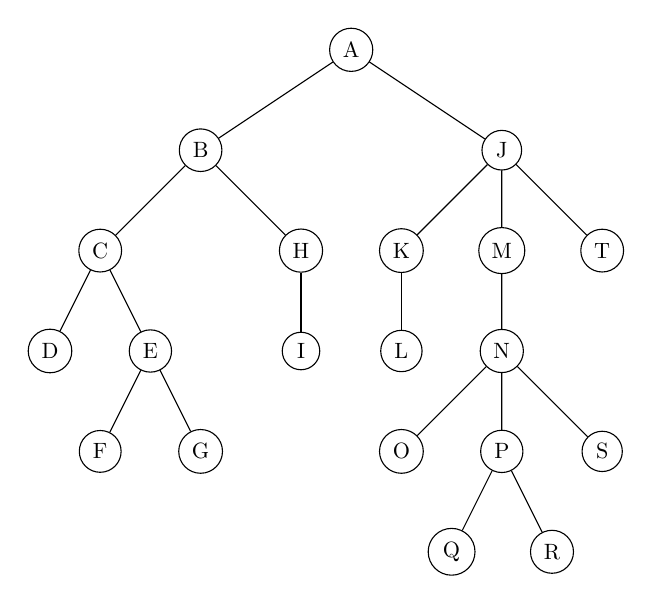
\begin{tikzpicture}[scale=0.85, every node/.style={scale=0.8}]
    \node [circle,draw] {A}
    child {node [circle,draw] {B}
        child {node [circle,draw] {C}
            child {node [circle,draw] {D}}
            child {node [circle,draw] {E}
                child {node [circle,draw] {F}}
                child {node [circle,draw] {G}}
            }
        }
        child [missing] {}
        child {node [circle,draw] {H}
            child {node [circle,draw] {I}}
        }
    }	
    child [missing] {}	
    child [missing] {}	
    child {node [circle,draw] {J}
        child {node [circle,draw] {K}
            child {node [circle,draw] {L}}
        }
        child {node [circle,draw] {M}
            child {node [circle,draw] {N}
                child {node [circle,draw] {O}}
                child {node [circle,draw] {P}
                    child {node [circle,draw] {Q}}
                    child {node [circle,draw] {R}}	
                }
                child {node [circle,draw] {S}}
            }
        }
        child {node [circle,draw] {T}}
    };
\end{tikzpicture}
\end{center}

\begin{parts}
    \part[2] The \textbf{children} of the \textbf{root node} with their \textbf{degree} respectively.
    \begin{solution}
        %%%%%%%%%%%%%%%%%%%%%%%%%%%%%%%%%%%%%%%%%%%%%%%%%
        % Replace `\vspace{2in}' with your answer.
        %\vspace{1in}
        B, J

        deg(B)=2, deg(J)=3
        %%%%%%%%%%%%%%%%%%%%%%%%%%%%%%%%%%%%%%%%%%%%%%%%%
    \end{solution}
    \part[2] All \textbf{leaf nodes} in the forest with their \textbf{depth} if we remove A and the node with the lexicographically smallest character in a tree is taken as the root node.
    \begin{solution}
        %%%%%%%%%%%%%%%%%%%%%%%%%%%%%%%%%%%%%%%%%%%%%%%%%
        % Replace `\vspace{2in}' with your answer.
        %\vspace{1in}
        D, F, G, I, L, O, Q, R, S, T

        height(T) = 1

        height(D) = height(I) = height(L) = 2

        height(F) = height(G) = height(O) = height(S) = 3

        height(Q) = height(R) = 4
        %%%%%%%%%%%%%%%%%%%%%%%%%%%%%%%%%%%%%%%%%%%%%%%%%
    \end{solution}
    \part[2] The \textbf{height} of the tree.
    \begin{solution}
        %%%%%%%%%%%%%%%%%%%%%%%%%%%%%%%%%%%%%%%%%%%%%%%%%
        % Replace `\vspace{2in}' with your answer.
        %\vspace{1in}
        height = max\{depth(v) | v \(\in\) V\} = 5

        so height = 5
        %%%%%%%%%%%%%%%%%%%%%%%%%%%%%%%%%%%%%%%%%%%%%%%%%
    \end{solution}

    \newpage

    \part[2] The \textbf{ancestors} of R. 
    \begin{solution}
        %%%%%%%%%%%%%%%%%%%%%%%%%%%%%%%%%%%%%%%%%%%%%%%%%
        % Replace `\vspace{2in}' with your answer.
        %\vspace{1in}
        R, P, N, M, J, A
        %%%%%%%%%%%%%%%%%%%%%%%%%%%%%%%%%%%%%%%%%%%%%%%%%
    \end{solution}
    \part[2] The \textbf{descendants} of L.
    \begin{solution}
        %%%%%%%%%%%%%%%%%%%%%%%%%%%%%%%%%%%%%%%%%%%%%%%%%
        % Replace `\vspace{2in}' with your answer.
        %\vspace{1in}
        L
        %%%%%%%%%%%%%%%%%%%%%%%%%%%%%%%%%%%%%%%%%%%%%%%%%
    \end{solution}
    \part[2] The \textbf{path} from E to S.
    \begin{solution}
        %%%%%%%%%%%%%%%%%%%%%%%%%%%%%%%%%%%%%%%%%%%%%%%%%
        % Replace `\vspace{2in}' with your answer.
        %\vspace{1in}
        \(E \to C \to B \to A \to J \to M \to N \to S\)
        %%%%%%%%%%%%%%%%%%%%%%%%%%%%%%%%%%%%%%%%%%%%%%%%%
    \end{solution}
\end{parts}